\documentclass[12pt]{article}
\usepackage{sbc-template}
\usepackage[alf]{abntex2cite} 
\usepackage{graphicx,url}
\usepackage[utf8]{inputenc}
\usepackage[brazil]{babel}
\usepackage{framed}                 %Incluindo Caixas
%\usepackage[latin1]{inputenc}      %Erro no inputenc.
\sloppy

\title{Mapeamento Sistemático sobre o uso do Learning Analytics na Aprendizagem Infantojuvenil com ênfase em Jogos}

\author{Alexandre Mendonça Fava\inst{1}}

\address{\inst{}Universidade do Estado de Santa Catarina - UDESC\\Programa de Pós-graduação em Computação Aplicada - PPGCA\\Joinville - SC - Brasil CEP: 89.219-710
    \email{\{alexandre.fava@hotmail.com\}}
}

\begin{document} 

\maketitle

\begin{resumo} 
%O ensino a distância é uma modalidade educativa em crescente expansão. Em 2020 o ensino a distância obteve um súbito crescimento em decorrência do novo coronavírus e da necessidade de contenção da doença. Neste contexto, as aulas presenciais passaram a ser ministradas a distância com base nas determinações do Ministério da Educação. O processo de ensino a distância gera uma quantidade superior de informações em relação ao ensino tradicional. Neste contexto, tem-se o  Learning Analytics para auxiliar no processo de análise dos dados escolares.Deste modo, este artigo apresenta um protocolo sobre um mapeamento sistemático da literatura na área de Learning Analytics.
A educação a distância é uma modalidade educativa em expansão. O processo de educação a distância gera uma quantidade superior de informações em relação ao ensino tradicional. O Learning Analytics é uma área de pesquisa relacionada à coleta e análise de dados dos alunos para o aprimoramento do aprendizado escolar. A área de Learning Analytics compreende inúmeras técnicas, objetivos e grupos. Nesse sentido, o presente artigo apresenta um mapeamento sistemático da literatura na área de Learning Analytics com ênfase em jogos no aprendizado de menores de idade (18 anos inclusive). O resultado final, é uma compilação acerca dos procedimentos, campos e instrumentos de maior relevância na área em questão.
\end{resumo}


\section{Introdução}\label{secao:introducao}

O uso das mídias digitais e dispositivos conectados a grande rede de computadores tem crescido desde o início da internet comercial no Brasil \cite{barbosa2019pesquisa}. %\footnote{Pesquisa sobre o Uso das Tecnologias de Informação e Comunicação nos Domicílios Brasileiros. Disponível: \url{https://cetic.br/media/docs/publicacoes/2/12225320191028-tic_dom_2018_livro_eletronico.pdf}}. 
Em 2020, a pandemia de COVID-19 foi responsável por um súbito crescimento nas plataformas de ensino a distância, tais como Google Classroom, Microsoft Teams e Blackboard Learn \cite{da2020inventar}. %\cite{barbosa2019pesquisa}

As plataformas de educação a distância demonstraram-se como uma alternativa viável na contenção e na propagação do vírus que causa a COVID-19 (SARS-CoV-2). A diminuição da circulação e do contato entre as crianças e jovens, no ambiente escolar, é uma atitude capaz de reduzir a taxa de contágio do vírus \cite{ferguson2020report}. 

Diferentemente das salas de aula tradicionais, as plataformas de ensino a distância permitem uma coleta mais automatizada e individualizada de algumas informações. Por exemplo: a verificação da presença dos alunos em uma determinada aula pode ser conferida nos arquivos de \textit{log} das plataformas, dispensando a necessidade de uma `chamada'.

As informações coletadas não se limitam apenas às informações nas quais os professores já poderiam coletar nas aulas tradicionais. As salas de aula virtuais permitem não apenas uma coleta mais automatizada, mas também uma coleta mais abrangente de informações, o que pode acabar dificultando o acompanhamento do professor em analisar todos os dados estudantis gerados pela plataforma \cite{de2019tendencias}. No mais, o sistema educacional atual não se limita apenas nas aulas com suas diapositivas e exercícios. O processo de educação abrange atualmente vários recursos e tecnologias, como por exemplo a área de jogos sérios \cite{educaccao2020ensino}.

%No mais, o sistema educacional não precisa se resumir em aulas online, com diapositivas disponíveis, professores sendo filmados e exercícios a serem feitos. As aulas podem se ramificar em outros campos, como por exemplo a área de jogos sérios \cite{educaccao2020ensino}.

Em vias de facilitar o processo de análise e compreensão dos dados estudantis, técnicas de Learning Analytics (LA) surgiram como um suporte para as tarefas de análise de aprendizagem virtual \cite{ruiperez2015alas}. O processo de LA busca coletar, medir, analisar e relatar os dados e seus contextos com objetivo de otimizar o aprendizado e o ambiente em que este ocorre \cite{moissa2015educational}. Percebe-se neste processo que os alunos obtêm abordagens customizadas para auxiliá-los a aprender e base de informação em um método que se encaixe às suas necessidades e não à classe toda.

\vspace{-0.1cm}

Apresentada a emersão das plataformas de educação digitais, e a importância do processo de LA para facilitar a ensino-aprendizagem, a atual pesquisa se objetiva a apresentar um panorama da área em questão com enfoque em jogos. O restante do trabalho está organizado da seguinte forma: na seção \ref{secao:trabalhos} são elencados alguns trabalhos relacionados, na seção \ref{secao:mapeamento} o mapeamento e seus processos são especificados, na seção \ref{secao:resultados} os principais achados são compilados e na seção \ref{secao:conclusao} são apresentadas as conclusões desta pesquisa. 

\vspace{-0.1cm}

\section{Trabalhos Relacionados}\label{secao:trabalhos}

\citeonline{moissa2014learning} realizaram um mapeamento sistemático na área de Learning Analytics. Ao total foram analisados 116 trabalhos compreendidos entre os anos de 2011 e 2014. %A coleta dos trabalhos se deu nos mecanismos de busca acadêmica: IEEE Xplore, ACM, Scopus e Science Direct (Elsevier). 
A análise dos trabalhos revelou que a coleta de dados mais utilizada na área de Learning Analytics se dá por meio de dados navegacionais, tais como tempo \textit{online} nas ferramentas e frequência de acesso. O histórico escolar das crianças também foi outra variável bem presente no mapeamento. %Dos trabalhos colhidos alguns eram exploratórios, outros apresentam propostas de ferramentas e apenas dois trabalhos apresentam ferramentas desenvolvidas.
Entre os achados, está a conclusão de que dados coletados de mídias sociais também podem auxiliar na melhor compreensão do comportamento dos alunos e auxiliar no gerenciamento da aprendizagem colaborativa.

\vspace{-0.1cm}

\citeonline{doko2018systematic} coletaram  122 artigos nas temáticas de Mineração de Dados na educação e Learning Analytics. %, das bases: IEEE Xplore, ACM, Springer e IJIRCCE. 
Um dos resultados diretos do artigo, foi a observação de um considerável crescimento da área entre os anos de 2010 e 2017. Entre os maiores achados, o mapeamento constatou uma crescente preferência por \textit{video segments} nas pesquisas. %Entre os maiores achados, está a observação do crescimento da dinâmica da sala de aula invertida no ensino superior desde 2012.

\vspace{-0.1cm}

\citeonline{de2018entrevistas} analisaram vários artigos em língua inglesa e portuguesa publicados após 2009, ao final 109 artigos foram analisados. %, os quais foram extraídos dos seguintes mecanismos de busca acadêmica: ACM, Science Direct (Elsevier) e IEEE Xplore. %A fonte da maioria dos artigos vem da International Conference on Learning Analytics and Knowledge (LAK).
Como resultado, foi constatado comparativamente que o objetivo da maioria dos artigos era o de identificar padrões de comportamento e trajetória dos alunos, sendo a matéria mais vista nesse contexto, a Informática. Matérias mais tradicionais como Matemática e Química não apresentaram larga presença no mapeamento realizado.

\vspace{-0.1cm}

Os trabalhos relacionados demonstram convergência no que diz respeito ao volume de artigos analisados. Do mesmo modo, os mapeamentos aqui elencados não relataram muitos jogos na área. Salienta-se que todos os trabalhos apresentados firmaram suas buscas nos buscadores acadêmicos da ACM e da IEEE Xplore. \citeonline{doko2018systematic} ainda afirmam que a maior parte dos trabalhos colhidos em sua pesquisa é oriunda destes buscadores. Em adendo, revisões sistemáticas da literatura realizadas especificamente na área de jogos sérios relatam também uma quantidade significativa de artigos encontrados nas bases da ACM, Science Direct (Elsevier) e IEEE Xplore \cite{calvo2020serious}. Nesse contexto, cita-se a revisão da literatura realizada por \citeonline{calvo2020serious}, a qual lista 31 artigos com o envolvimento de crianças. Por tal razão, se espera que a quantidade de artigos elencadas neste mapeamento seja próxima deste valor.

%O estudo realizado sobre os trabalhos relacionados permite observar uma provável duplicação parcial de seus resultados. Cabe ressaltar que há diferença nas frases de busca utilizadas pelos mapeamentos, assim como a escolha por outros mecanismos de busca acadêmicas. Contudo, salienta-se que os termos ``\textit{data mining}'' e ``\textit{learning analytics}'' compuseram as frases de busca de todos os trabalhos relacionados aqui elencados. 


\section{Mapeamento Sistemático}\label{secao:mapeamento}

Mapeamentos sistemáticos são projetados para dar um panorama geral de uma determinada área, envolvendo uma busca na literatura para descobrir os estudos primários que foram publicados em um tema de pesquisa \cite{chen2017science}. O mapeamento se diferencia da revisão sistemática, a qual avalia a força das evidências. O processo se divide em: definir uma pergunta de pesquisa, definir palavras-chave, selecionar os estudos, extrair os dados, analisar, classificar e validar \cite{khan2003five}. 

O presente trabalho realiza um mapeamento sistemático na área de Learning Analytics para o ensino infantil com foco na temática de jogos. A área de jogos foi eleita para o presente mapeamento, uma vez constatada sua fraca presença no estudo dos trabalhos relacionados (Seção \ref{secao:trabalhos}). Deste modo, busca-se ampliar a visão geral da área de LA no campo dos jogos para a educação infantojuvenil. 

Os passos necessários para a execução de um mapeamento sistemático na área de LA para a educação infantojuvenil na temática de jogos é descrito mais detalhadamente em suas subseções: a subseção \ref{a:1} apresenta as questões de pesquisa, a subseção \ref{a:2} mostra a frase de busca, a subseção \ref{a:3} define os critérios objetivo para inclusão e exclusão de artigos, assim como o critério de parado do presente mapeamento.

%Segundo \cite{petersen2015guidelines}, um mapeamento é um processo para classificação e contabilização das contribuições existentes em uma determinada área.  Ou seja, o mapeamento permite a estruturação da área de pesquisa a ser realizada,bem como expor uma nova visão para área e indicar as tendências de pesquisas.

\vspace{-0.1cm}

\subsection{Questões de Pesquisa}\label{a:1}

\vspace{-0.1cm}

O primeiro passo para a execução de qualquer mapeamento sistemático é a definição das questões de pesquisa. Essas questões de pesquisa são responsáveis por ditar o que se espera conseguir do mapeamento sistemático. As questões que norteiam o atual mapeamento sistemático são:

\vspace{-0.1cm}

\begin{enumerate}
    \item Quais os tipos de dados coletados?
    \item Quais são os tamanhos das amostras nos estudos?
    \item Quais são as disciplinas mais presentes nos estudos?
    \item Quais métodos são utilizados para analisar os alunos?
    \item Quais ferramentas são utilizadas para analisar as informações dos estudantes?
\end{enumerate}

\vspace{-0.1cm}

A \textbf{primeira questão} busca identificar as variáveis que mais se destacam no âmbito investigado. A primeira questão, se mescla um pouco com a \textbf{quinta questão}, a qual versa sobre as tecnologias utilizadas para coletar as variáveis mensuradas pelos estudos. Do mesmo modo, a \textbf{quarta questão} assume uma posição equivalente visando identificar as estratégias utilizadas para se trabalhar com os dados colhidos. Por fim, a \textbf{segunda questão} de pesquisa e a \textbf{terceira questão} de pesquisa assumem características mais triviais, as quais possibilitam a identificação não apenas da extensão dos grupos avaliados nas pesquisas, mas também das matérias escolares mais presentes neste âmbito. 


\subsection{Frase de Busca}\label{a:2}

\vspace{-0.1cm}

Após a definição das questões de pesquisa é necessário estabelecer as bases de dados acadêmicas que serão utilizadas. \citeonline{buchinger2014mecanismos} realizaram uma análise quantitativa com 40 Mecanismos de Busca Acadêmicas. Para a execução de uma pesquisa científica é recomendado a utilização de pelo menos três fontes de dados distintas. Para o presente mapeamento, quatro bases foram utilizadas: ACM, DBLP, IEEE Xplore e Science Direct (Elsevier). As bases elencadas, além de serem bons buscadores de acordo com a pesquisa de \citeonline{buchinger2014mecanismos}, também estão em conformidade com as relatadas nos trabalhos relacionados (Seção \ref{secao:trabalhos}).

A realização de uma pesquisa nos mecanismos de busca acadêmicas, pode ser realizada com maior precisão com o auxílio de alguns recursos de busca disponíveis como caractere coringa e operadores booleanos. A busca deve ser realizada nas palavras-chave, título e resumo do artigo preferencialmente. Salienta-se que algumas ferramentas de busca estão limitadas a um conjunto máximo de oito operadores booleanos (como o Science Direct). O presente mapeamento formulou uma frase de busca simples com o intuito de respeitar as limitações de todos os mecanismos de busca utilizados: 

\begin{framed}
 %\raggedright (``e-learning Analytics'' OR ``elearning Analytics'' OR ``Learning Analytics'') \\ AND (chil* OR kid* OR infant* OR minor*) AND game
 \centering ``Learning Analytics'' AND children AND game
\end{framed}

\vspace{-0.25cm}

A frase de busca utilizada apresenta de maneira simples e em língua inglesa os três termos de maior relevância para o presente mapeamento. Notoriamente, sabe-se que existem outras palavras (sinônimos) para os termos elencados, contudo constatou-se em um primeiro momento conflito na formatação do operador OR entre alguns mecanismos, deste modo optou-se em utilizar apenas o operador lógico AND, o qual permitiu a construção de uma frase de busca invariável entre os mecanismos de busca acadêmica utilizados. Além disso, os termos elencados não fogem do escopo, abrangendo área, técnica e grupo, como recomendado por \citeonline{wazlawick2009metodologia}. O total de publicações retornadas é apresentado detalhadamente na Tabela \ref{tab:numero}.

{\centering
\captionof{table}{Quantidade de publicações retornadas por Mecanismo de Busca}\label{tab:numero}
\begin{tabular}{l*{1}c}
\textbf{Mecanismo de Busca}              & \textbf{Quantidade} \\
\hline
ACM  & 130   \\
DBLP            & 1   \\
IEEE Xplore           & 2   \\
Science Direct (Elsevier)    & 44   \\
\hline
\textbf{Total}           & 177
\end{tabular}\par
}

A busca realizada nos mecanismos elencados retornou um total de 177 resultados. Informa-se nesse sentido que a busca foi realizada no mês de agosto de 2020. Buscas realizadas em uma janela de tempo superior a este período tendem a retornar quantidades cada vez mais diferentes no número de resultados na medida que a data buscada for se afastando da data de busca realizada pela presente pesquisa. Afim de trazer maior transparência aos procedimentos deste mapeamento, enfatiza-se que as páginas dos resultados da busca foram gravadas em PDF e encontram-se disponível a qualquer um que queira requisitá-las para conferir os vereditos desta pesquisa. 

%As páginas retornadas com a lista dos resultados foram gravadas em um Formato Portátil de Documento. A gravação dos resultados retornados em PDF é devido a inviabilidade de exportação dos resultados para o formato BibTeX por parte dos mecanismos de busca utilizados.


\subsection{Critérios Objetivos}\label{a:3}

A execução da busca dos artigos e demais pesquisas nas bases de dados acadêmicas pode retornar trabalhos indesejados para o mapeamento sistemático. Deste modo surgem os critérios de inclusão e exclusão com o objetivo de ajudar a descartar os artigos que, embora contivessem as palavras-chave definidas na frase de busca, não contribuíam para responder as questões de pesquisa. Como critérios de inclusão estabelece-se:

\begin{itemize}
    \item Pesquisas publicadas após 2010, inclusive.
    \item Pesquisas de acesso livre e gratuito.
    \item Pesquisas envolvendo menores.
    \item Pesquisas utilizando jogos.
    \item Pesquisas primárias.
\end{itemize}

Informa-se que o critério do \textbf{ano da publicação} foi o único já englobado no momento da busca, devido a existência de recursos de seleção por período nos mecanismos utilizados. Salienta-se então que todos os 177 artigos retornados pelas bases acadêmicas são de uma data superior ao ano de 2010, inclusive. Este critério vem com o intuito de excluir pesquisas mais antigas, sendo o objetivo do presente mapeamento uma apresentação mais atual do estado da arte da área e também das tecnologias mais recentes utilizadas. 

A \textbf{disponibilidade} das publicações é um critério importante, o qual permite que os resultados apresentados por esse mapeamento possam ser mais facilmente acessados. A participação de \textbf{menores} (indivíduos de até 18 anos) é outro critério necessário para o presente mapeamento, uma vez que existe a possibilidade de pesquisas conterem o termo `\textit{children}' em algum dos campos buscados, sem que estas tenham de fato a participação ou o envolvimento de crianças ou jovens, o mesmo se faz válido no que diz respeito a utilização de \textbf{jogos} na pesquisa. 

O último critério de inclusão, diz respeito a contribuição do artigo. Deste modo, o presente mapeamento valoriza as \textbf{pesquisas primárias}, as quais apresentam novos resultados e experimentos. Todos os critérios de inclusão devem ser verdadeiros para que um artigo seja considerado viável para ser incluído no mapeamento sistemático. Contudo, basta um critério de exclusão ser constatado para uma pesquisa ser descartada. Como critérios de exclusão elencam-se: 

\begin{itemize}
    \item Pesquisas duplicadas.
    \item Pesquisas não escritas em inglês.
    \item Pesquisas sem os termos da frase de busca no título, resumo ou palavra-chave.
\end{itemize}

A preferência de pesquisas em \textbf{língua inglesa}, se deve pelo fato deste idioma apresentar a maior quantidade de publicações acadêmicas do ocidente, em comparação a qualquer outro idioma, o que amplia a quantidade de pesquisas retornadas. A exclusão de \textbf{pesquisas repetidas} visa trazer uma melhor acurácia aos numerativos apresentados pelo presente mapeamento, já os campos utilizados para a busca visam trazer maior agilidade para o processo de seleção e qualificação dos artigos, uma vez que todos os processos do presente mapeamento sistemático foram executados por somente um indivíduo. Em adendo, salienta-se que todo o protocolo do mapeamento, tanto quanto seus resultados foram validados pelos orientadores do presente pesquisador. 

As 177 publicações retornadas tiveram seus títulos, resumos, introduções e conclusões (quando existentes) lidas de modo a incluir ou excluir uma determinada pesquisa do mapeamento. Nenhum critério de priorização por \textit{Qualis}, veículo de publicação ou quantidade de referências foi aplicado, garantindo a leitura de todas as 177 pesquisas. 

Durante o processo de leitura, algumas publicações de revisão da literatura na área foram descobertas \cite{calvo2020serious, alonso2019applications}. Salienta-se que no decorrer do processo, não houve nenhuma inclusão Ad-hoc e também não foi realizada nenhuma pesquisa ao entorno, tudo isso para garantir e preservar o rigor do processo sistemático do mapeamento. Deste modo, o critério de parada do presente mapeamento foi atingido com a finalização da leitura dos 177 trabalhos, restando 29 artigos ao final. O resultado compilado dos numerativos de exclusão é apresentado de maneira geral na Figura \ref{fig:excluidos}. A Tabela \ref{tab:aprovados} apresenta a relação das pesquisas remanescentes por mecanismo de busca. 

\newpage

{\centering
\captionof{table}{\raggedright Publicações qualificadas}\label{tab:aprovados}
\begin{tabular}{l*{1}c}
\textbf{Mecanismo de Busca}              & \textbf{Qualificados} \\
\hline
ACM  & 20   \\
DBLP            & 1   \\
IEEE Xplore           & 1   \\
Science Direct (Elsevier)    & 7   \\
\hline
\textbf{Total}           & 29
\end{tabular}
}

\begin{figure*}[ht]
\vspace{-5.0cm}
\hspace{7.1cm}
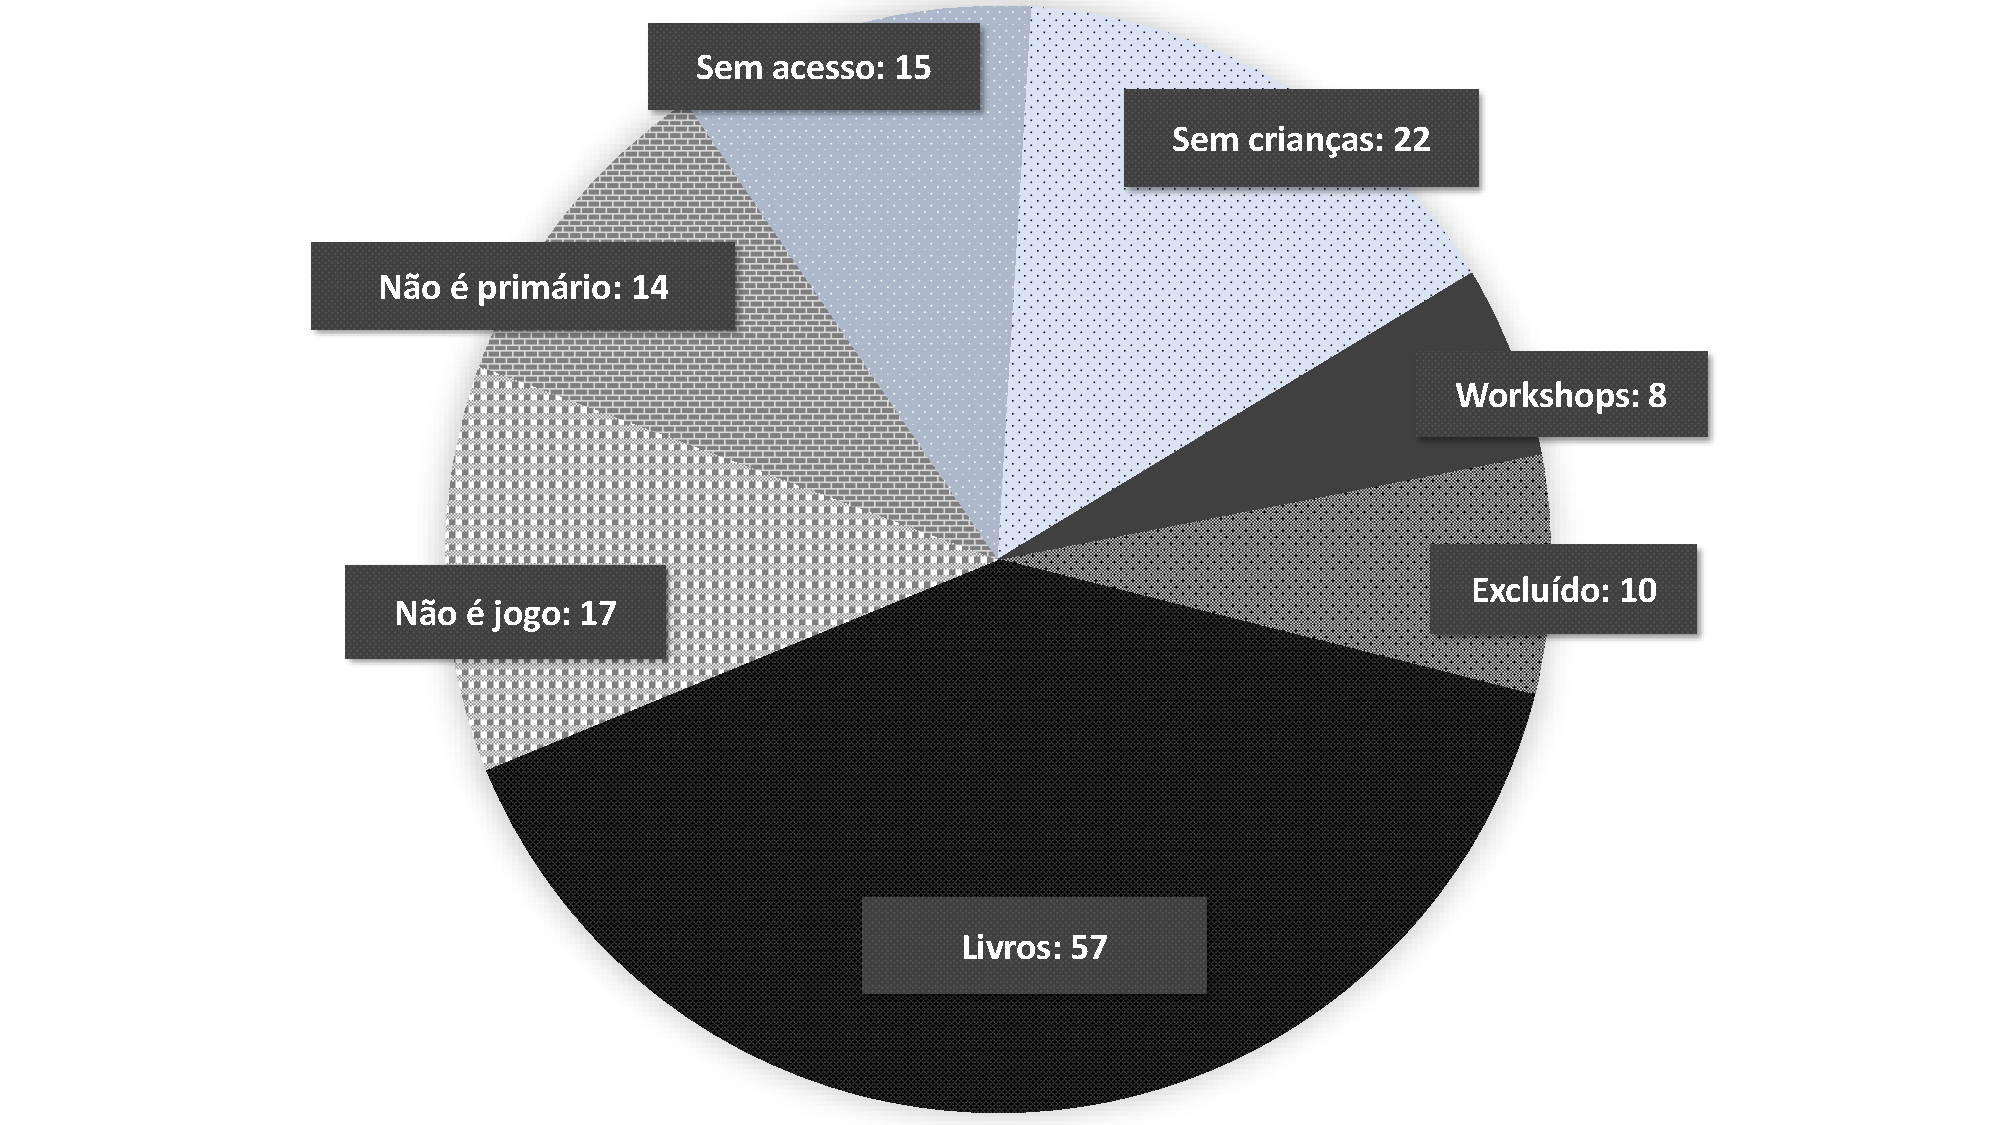
\includegraphics[width=0.65\textwidth]{Figuras/Excluidos.pdf}
\caption{\raggedleft Publicações excluídas}\label{fig:excluidos}
\end{figure*}

A Figura \ref{fig:excluidos} apresenta um gráfico circular com os quantitativos das publicações excluídas após a etapa de leitura do protocolo de mapeamento. Cerca de 33\% (57) das publicações retornadas eram livros, 13\% (22) não apresentavam o envolvimento de crianças na pesquisa, 10\% (17) não utilizavam jogos, 9\% (15) não eram acessíveis, 8\% (14) não eram pesquisas primárias, 4\% (8) eram Workshops e 6\% (10) foram excluídos por não conterem os termos buscados nos campos designados. Ao final, 17\% (29) foram validados pelo processo de leitura.

Todas as etapas do presente mapeamento foram executadas sem conflitos de interesse. A agência financiadora da presente pesquisa (CAPES) dá livre liberdade de expressão, manifestação e pesquisa para seus bolsistas. Contudo, salienta-se que o atual mapeamento (executado com protocolo bem definido e seguido rigorosamente) não é imune a falhas. Eventuais equívocos ou descuidos podem ter ocorrido durante o processo, no que diz respeito a validade interna e externa do mapeamento. 

Os problemas de validade externa podem ter ocorrido devido à falta de padronização em alguns termos utilizados nas frases de busca. Sabe-se que o termo mais academicamente aceito para jogos no contexto educacional é a terminologia ``jogo sério'', cunhada em 2002 \cite{djaouti2011origins}. Entretanto, pesquisas mais recentes continuam a utilizar outros termos, uma vez que não houve a padronização da terminologia. Afirma-se que a palavra ``jogo'' encontra-se presente também nas demais terminologias, por tal razão acredita-se que os problemas de integridade externa tenham sido minimizados nesse sentido. 

Os problemas de integridade interna podem ser inúmeros. No contexto desta pesquisa o problema de maior destaque nesse sentido, vem no momento da apresentação dos grupos avaliados em determinados trabalhos. Grande parte dos trabalhos definiam claramente um limite inferior e superior da idade dos participantes da pesquisa, o que ajuda na condensação dos dados para o presente mapeamento. Todavia, um conjunto de trabalhos apresentava a idade dos participantes de maneira indireta, mencionando suas turmas ou classes de aula por exemplo. A falta de clareza neste sentido, foi um dos fatores que contribuíram para possíveis problemas de integridade interna no mapeamento realizado. 

Todo o processo de seleção, leitura, coleta e análise dos trabalhos foi realizado no período de um mês. A execução do protocolo de mapeamento e a escrita do presente artigo foi realizada por um bolsista da CAPES. Salienta-se novamente que o protocolo de mapeamento foi validado pela orientadora e coorientador do presente autor. 

\section{Resultados e Análise}\label{secao:resultados}

O último passo para o mapeamento sistemático é o de analisar o conteúdo dos artigos restantes, encontrando relações, achados importantes e respondendo as questões de pesquisa formuladas. Durante esse processo artigos podem ser descartados, mas não incluídos. A leitura completa dos 29 artigos restantes foi realizada, nesse processo nenhum artigo foi excluído. A separação dos artigos por veículo de publicação é mostrada na Figura \ref{fig:LocaisPublicacao}. Já a dispersão temporal de todos os artigos é apresentada mais detalhadamente na Figura \ref{fig:AnoPublicacao}.

\begin{figure*}[!htb]
    \centering
    \begin{minipage}{.5\textwidth}
        \centering
        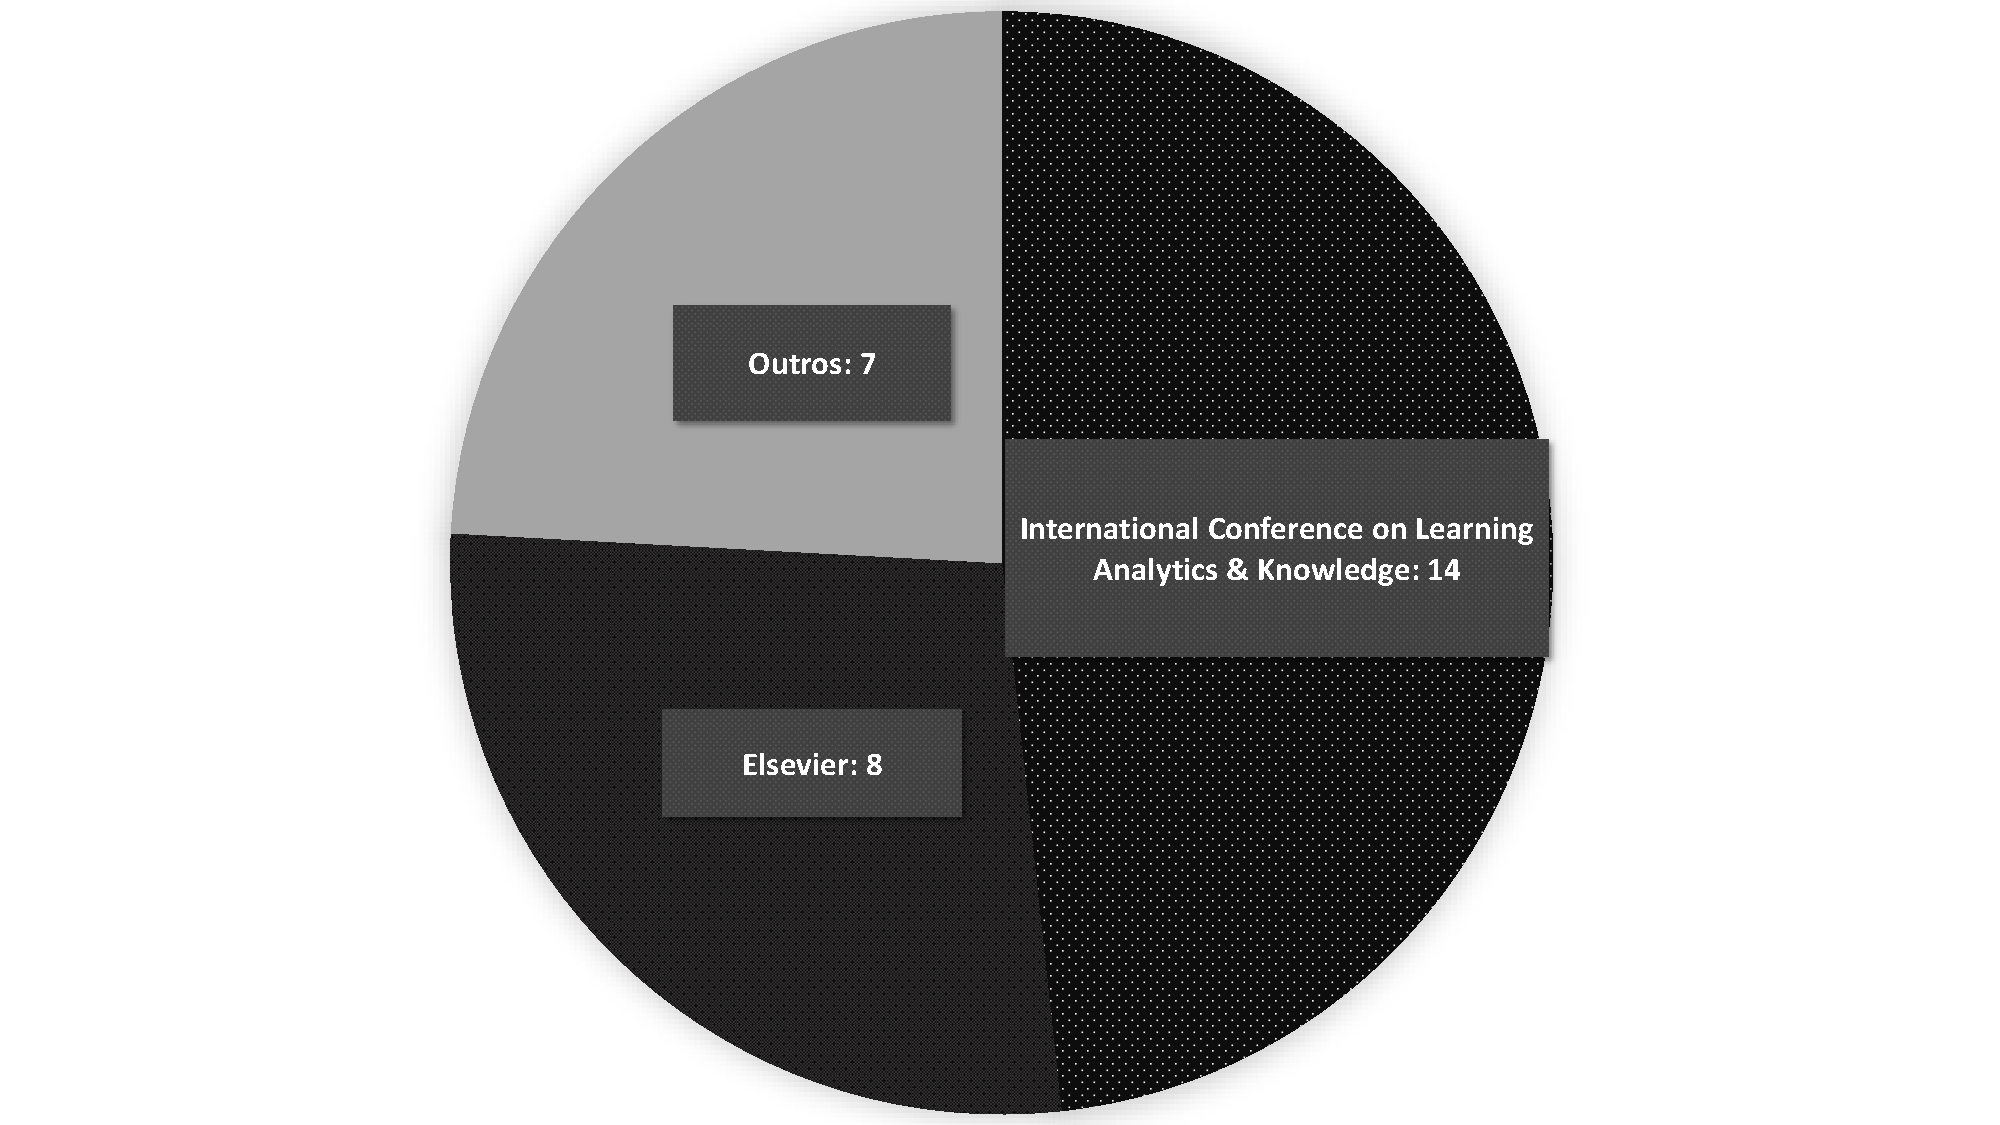
\includegraphics[width=\linewidth]{Figuras/LocaisPublicacao.pdf}
        \caption{Separação dos artigos por local de publicação}\label{fig:LocaisPublicacao}
    \end{minipage}%
    \begin{minipage}{0.5\textwidth}
        \centering
        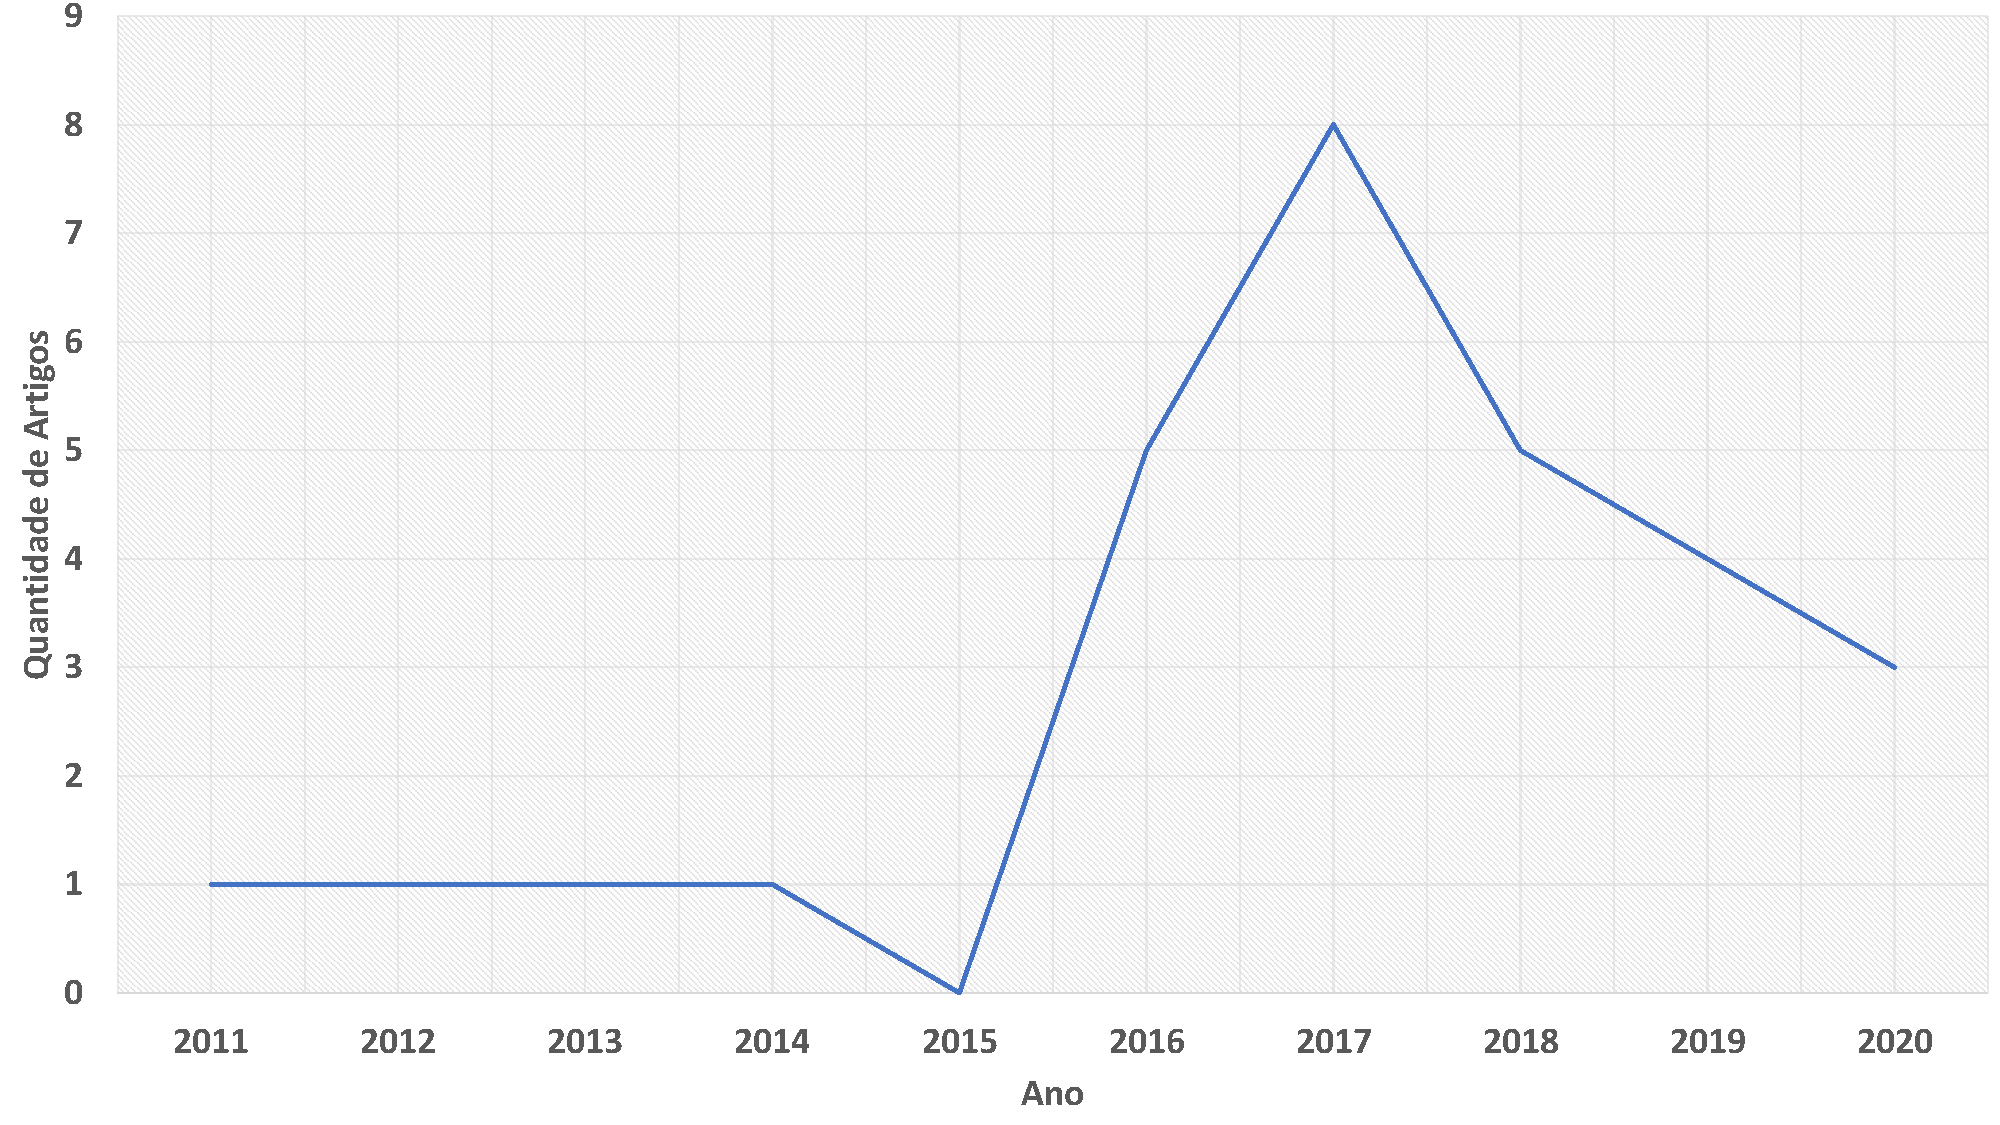
\includegraphics[width=\linewidth]{Figuras/AnoPublicacao.pdf}
        \caption{Quantidade de artigos por ano de publicação}\label{fig:AnoPublicacao}
    \end{minipage}
\end{figure*}

%Gráficos de bolhas, barras ou tabelas, são úteis para uma rápida compreensão das relações existentes na área estudada. Um esquema relacionando o tempo corrido e o número de publicações é excelente para identificar tendências. A análise dos artigos deve ser feita de modo a presar a responder as questões de pesquisa, no entanto, outras questões respondidas podem ser apresentas, tal como relações encontradas ou fatos interessantes na área. 

A Figura \ref{fig:AnoPublicacao} demonstra um considerável crescimento de estudos que relacionam jogos e Learning Analytics com o envolvimento de menores após 2015. Reitera-se nesse sentido que os dados para o ano de 2020 vão somente até o mês de agosto, o que resulta um quantitativo incompleto para o ano em questão. A Figura \ref{fig:LocaisPublicacao} apresenta os locais onde as pesquisas foram publicadas. A conferência de maior destaque nesse contexto é a \textit{International Learning Analytics and Knowledge Conference}. Outras conferências também marcaram presença no presente mapeamento, como a \textit{International Conference on Interaction Design and Children} e a \textit{Conference on Innovation and Technology in Computer Science Education}.

A quantidade de participantes evolvidos nos estudos apresentou grande flutuação. Os maiores numerativos nesse sentido foram de pesquisas que se utilizaram de bases de dados já existentes. A maior base utilizou dados de mais de 300.000 crianças, tais dados foram extraídos do sistema Todo Math\footnote{Todo Math é um aplicativo de aprendizagem baseado em dispositivos móveis que contém conceitos matemáticos básicos para crianças nas fases iniciais do ensino fundamental.} \cite{kim2018ll}. O menor numerativo encontrado durante o mapeamento foi de um \textbf{estudo de caso} que acompanhou por cinco dias uma única menina de dez anos de idade \cite{pantic2016studying}. 

Mais de 50\% das pesquisas avaliaram grupos de dez até sessenta indivíduos. Cerca de 18\% avaliaram grupos de 100 até 500 indivíduos. Pouco mais de 10\% avaliaram grupos menores de 10 indivíduos. Os 12\% restantes se enquadram em outros numerativos. Metade dos trabalhos informaram as dimensões de seus grupos por gênero. Com a exceção de quatro artigos, todos os demais relataram as faixas etárias dos grupos avaliados. O gráfico de barras da Figura \ref{fig:IdadeParticipantes} mostra a dispersão por idade dos estudos.

\pagebreak

\begin{figure*}[ht]
\centering
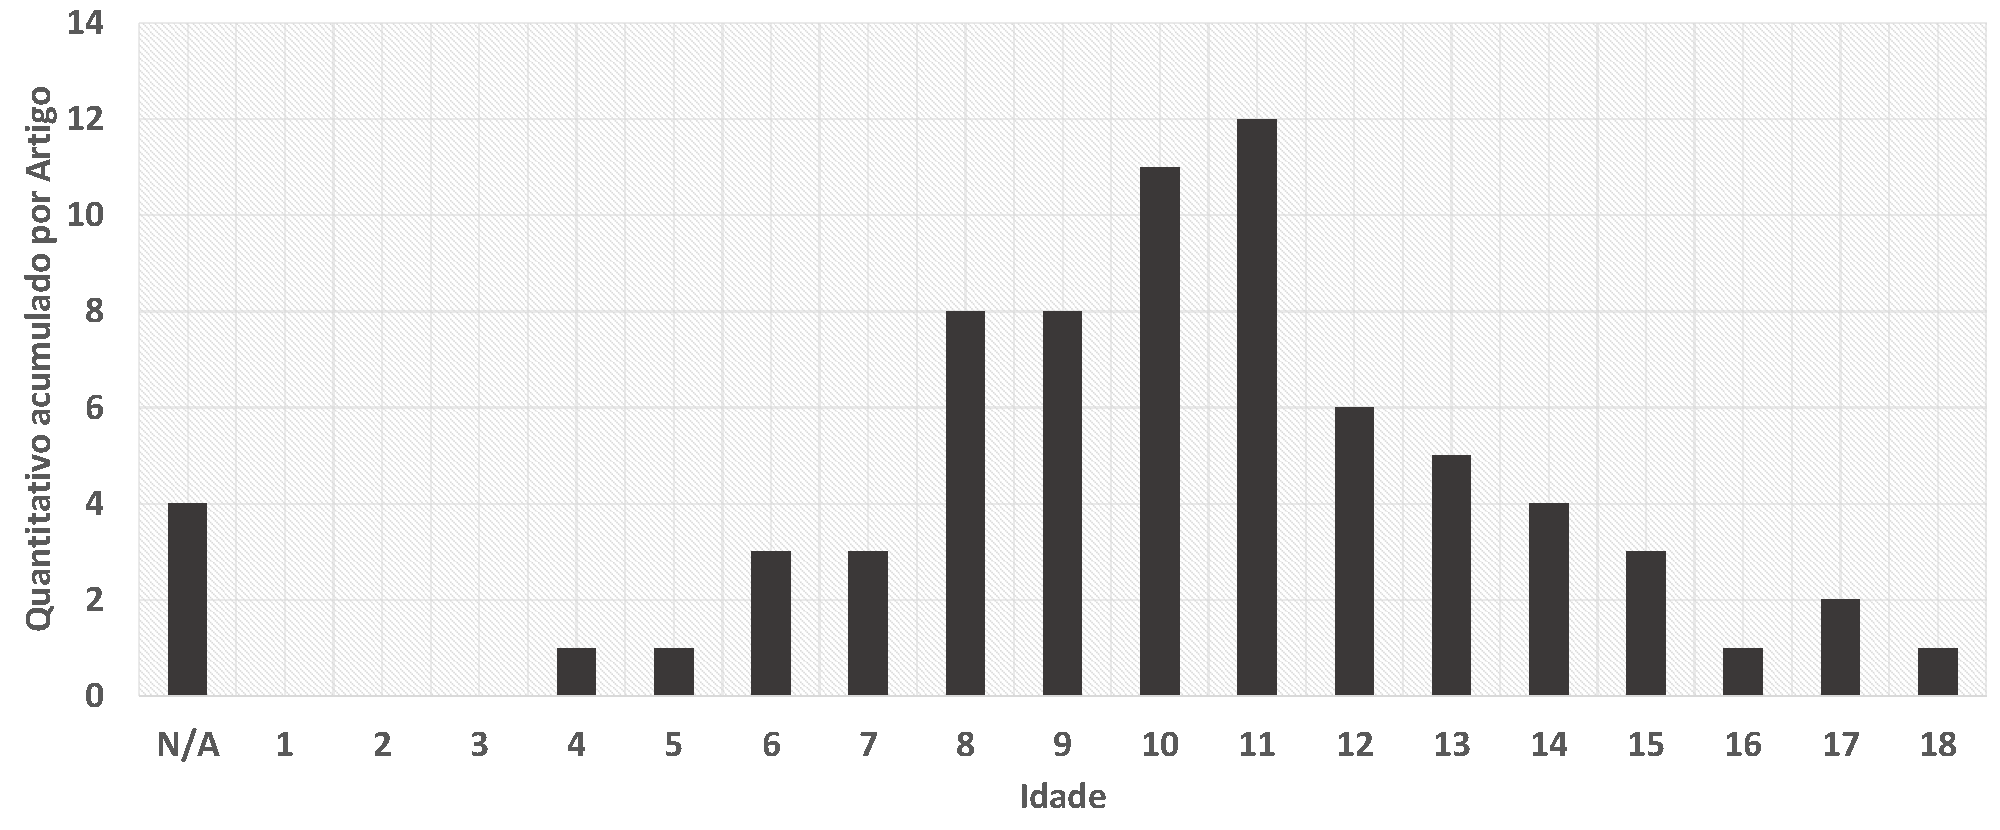
\includegraphics[width=0.94\textwidth]{Figuras/IdadeParticipantes.pdf}
\caption{Distribuição da idade dos participantes dos artigos}\label{fig:IdadeParticipantes}
\end{figure*}

A Figura \ref{fig:IdadeParticipantes} apresenta a variação de idade encontrada ao longo do presente mapeamento. A sigla \textbf{N/A} (Não se Aplica) representa os artigos nos quais não foi possível mensurar a faixa etária dos envolvidos no estudo. Parte dos trabalhos relatavam somente o ano letivo dos participantes, onde a idade dos participantes só foi possível mensurar de maneira indireta. Os trabalhos relatados em \textbf{N/A}; ou não apresentavam nenhum informativo do qual a informação da idade dos participantes poderia ser inferida; ou relatavam dados imprecisos (contudo, foi possível inferir que tratavam-se de menores de 18 anos).%, como por exemplo: informar que os participantes eram do ensino fundamental.

A distribuição etária da Figura \ref{fig:IdadeParticipantes} mostra uma distribuição normal, onde a faixa etária de maior destaque é a faixa dos onze anos de idade. Salienta-se que os intervalos etários convergiam entre algumas pesquisas, por tal razão o numerativo total da distribuição etária é superior a quantidade total de artigos avaliados. As exceções ocorrem nos artigos que não mencionaram um intervalo da idade, mas sim, a média de idade dos participantes. É importante destacar que os baixos numerativos nas extremidades do gráfico podem ter ocorrido em virtude dos termos utilizados na frase de busca, sendo o termo \textit{toddler} o mais apropriado para descrever as crianças de zero até três anos de idade e o termos \textit{teenager} ou \textit{adolescent} para as de treze até dezenove anos. 

A distribuição etária reflete nas temáticas dos jogos presentes nos estudos e nas variáveis coletadas, tais quantitativos podem ser observados mais detalhadamente na Figura \ref{fig:AssuntosPublicacao} e na Figura \ref{fig:ObjetoEstudo}.


\begin{figure*}[!htb]
    \centering
    \begin{minipage}{.5\textwidth}
        \centering
        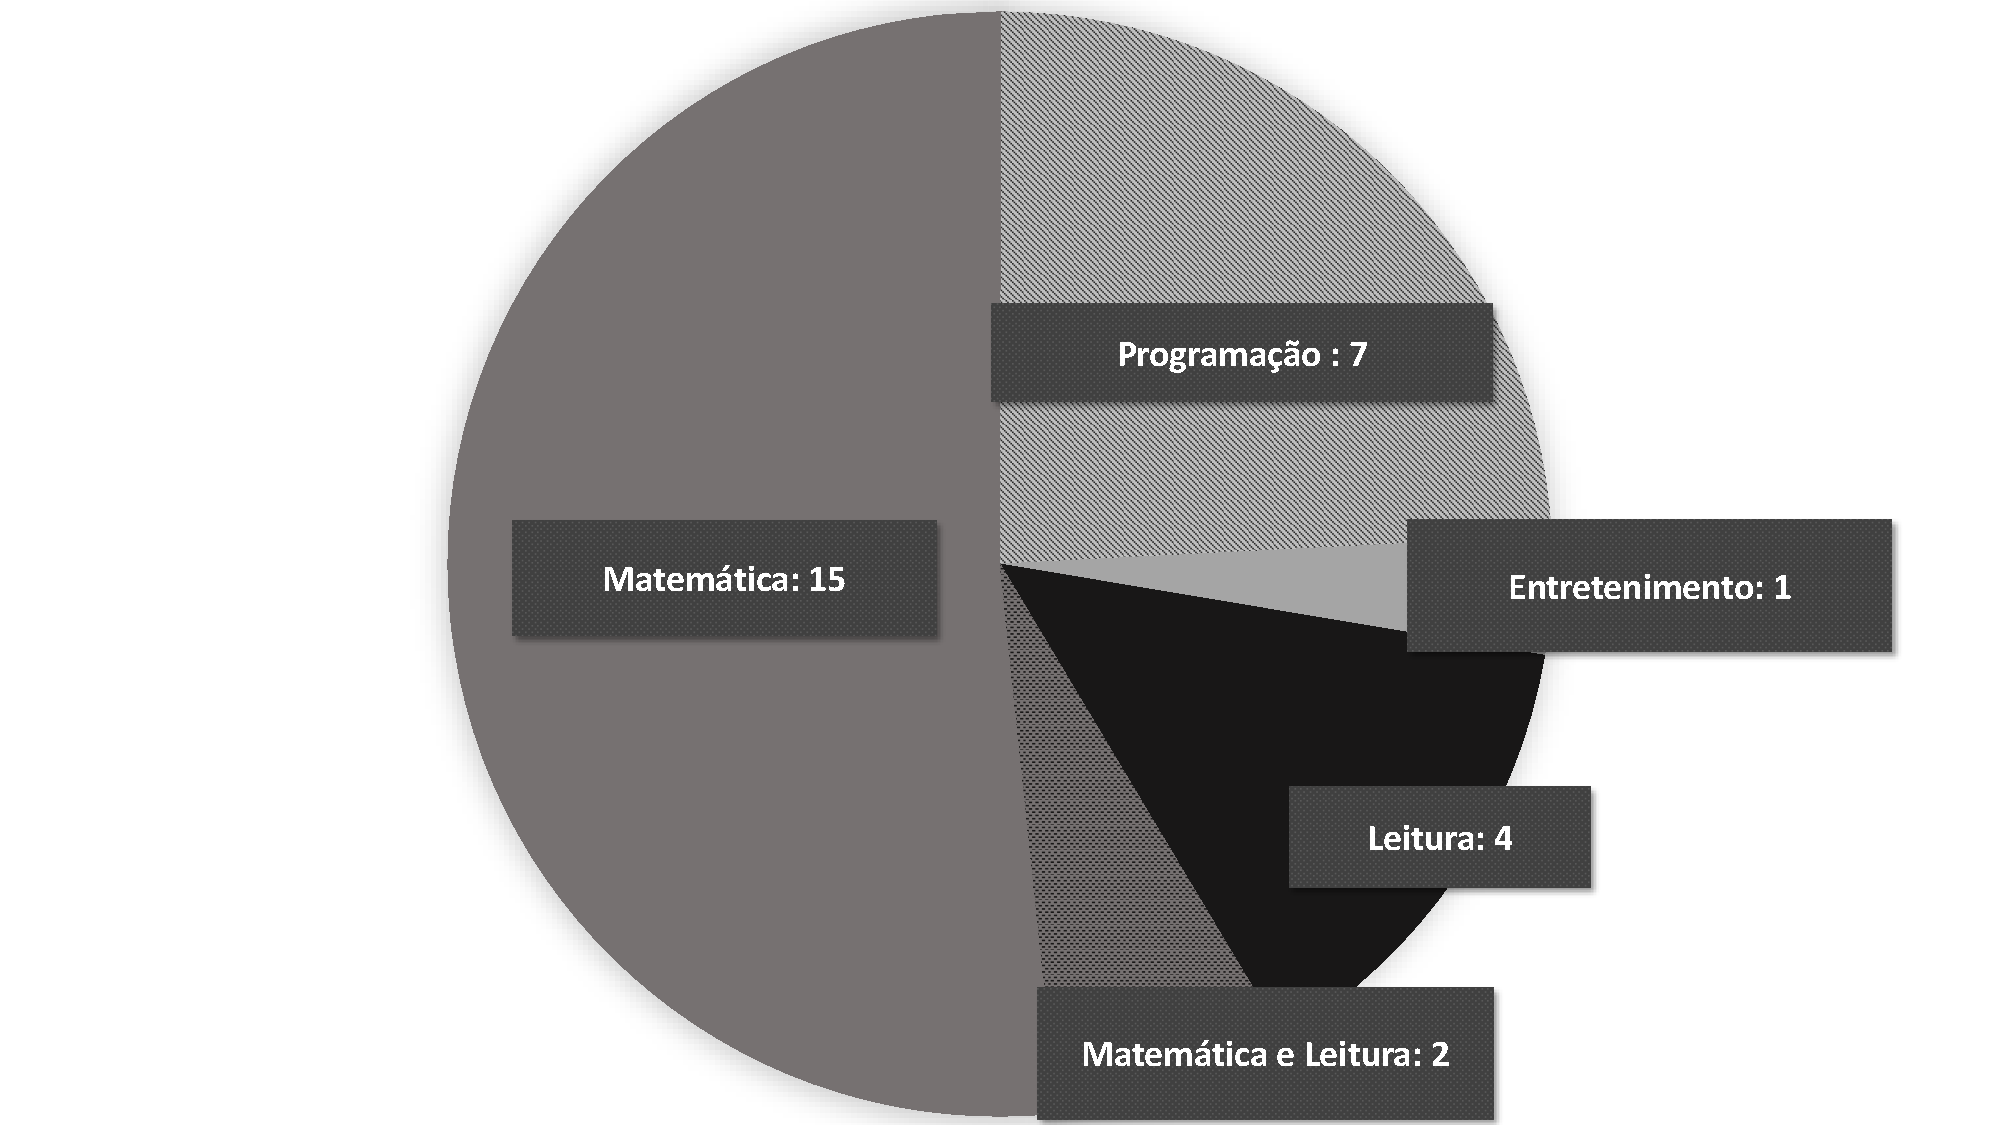
\includegraphics[width=1.1\linewidth]{Figuras/AssuntosPublicacao.pdf}
        \caption{Artigos por assunto}\label{fig:AssuntosPublicacao}
    \end{minipage}%
    \begin{minipage}{0.5\textwidth}
        \centering
        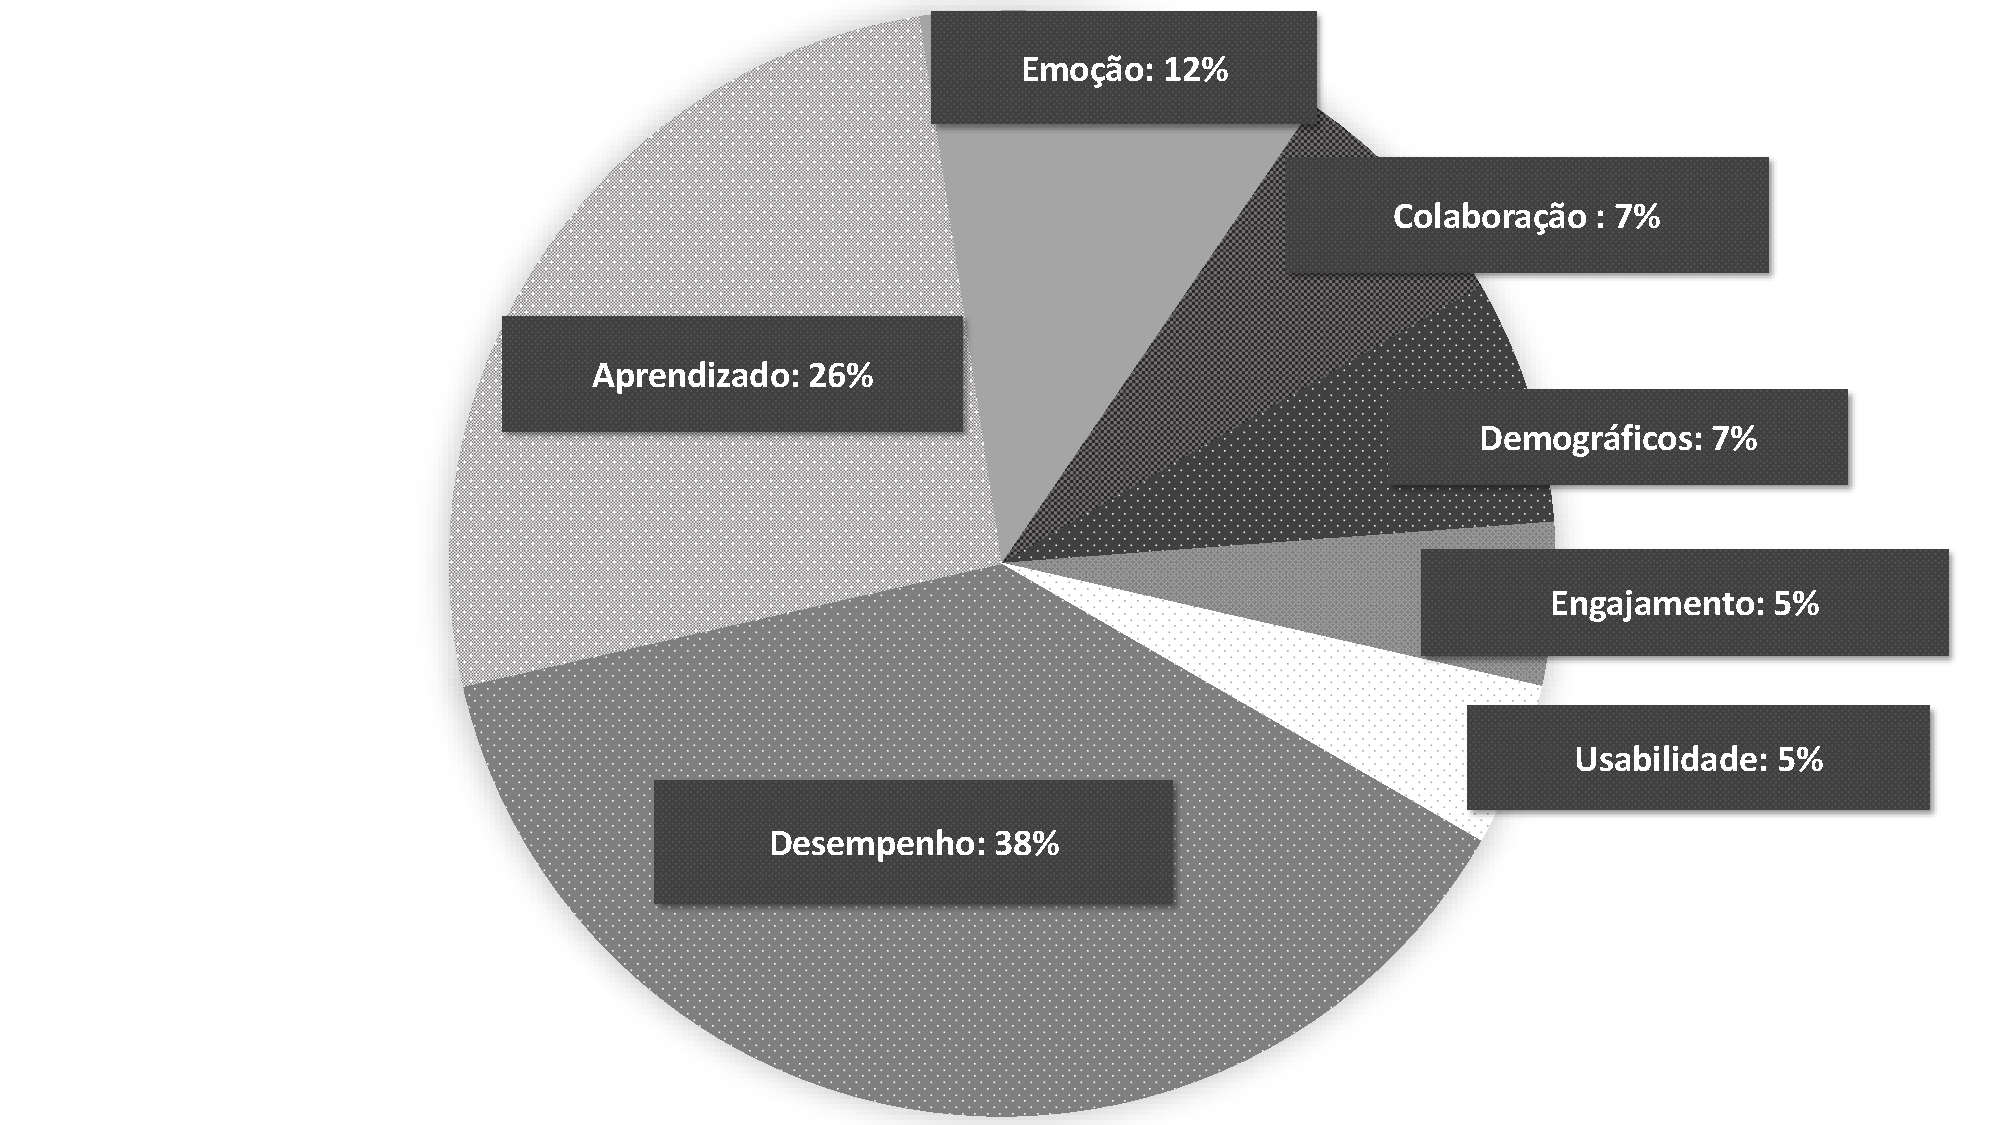
\includegraphics[width=1.15\linewidth]{Figuras/ObjetoEstudo.pdf}
        \caption{Percentual das variáveis mensuradas nos artigos}\label{fig:ObjetoEstudo}
    \end{minipage}
\end{figure*}

A Figura \ref{fig:AssuntosPublicacao} mostra as principais temáticas dos jogos no mapeamento realizado. Grande maioria dos jogos eram de propósito didático, a exceção está na pesquisa de \citeonline{tsuei2019preliminary} que realizou uma avaliação de usabilidade de  um jogo de entretenimento VR (Realidade Virtual). A Figura \ref{fig:ObjetoEstudo} condensa as variáveis de maior expressão mensuradas pelos estudos. Salienta-se que grande parte das pesquisas relacionavam duas ou mais variáveis, sendo a relação de maior destaque a variável de \textbf{desempenho} das crianças no jogo com a variável de \textbf{aprendizado} dos conteúdos no âmbito escolar. 

Para coletar e mensurar as variáveis, inúmeras técnicas foram utilizadas pelos estudos. A grande maioria se utilizaram de \textit{log de dados} (14 artigos). Coletas de áudio e vídeo também estiveram presentes em alguns estudos (8 artigos). A utilização de testes também é relatada em algumas pesquisas (20 artigos), porém uma quantidade menor de pesquisas relataram a aplicação tanto de pré, quanto de pós-testes (10 artigos), além disso, um numerativo reduzido de artigos informaram se utilizar de um grupo controle para isolar variáveis (6 artigos). Da mesma forma, poucas pesquisas relataram a utilização de \textit{hardwares} ou \textit{softwares} mais avançados para a coleta ou análise das variáveis (4 artigos), tais como: Eye-Tracking, Wristband, FaceReader e Kinect.


\section{Conclusão}\label{secao:conclusao}

Neste trabalho foi realizado um mapeamento sistemático conduzido nas bases acadêmicas ACM, DBLP, IEEE Xplore e Science Direct (Elsevier). Ao total 177 publicações foram retornadas; após a filtragem das publicações, 29 artigos remanesceram. Os artigos restantes permitiram identificar quais são os dados mais almejados pelas pesquisas na área da educação infantil e juvenil com auxílio de jogos. Tais dados, precisam ser coletados e devidamente analisados, deste modo surge o Learning Analytics que tem como objetivo melhorar o processo de ensino-aprendizagem por meio da análise de dados estudantis. Dentre as informações mais almejadas pelas pesquisas estão: a coleta de relatório de desempenho, aprendizado e emoções. Isso permite responder a primeira questão de pesquisa do presente mapeamento. 

A coleta das variáveis pode ser realizada de inúmeras maneiras, nos artigos elencados as formas de coleta mais presentes nos estudos são: coleta por \textit{log de dados}, materiais audiovisuais e testes/provas. Isso permite responder a quinta questão de pesquisa deste mapeamento. Informa-se que tal achado está em consonância com a pesquisa de \citeonline{moissa2014learning}, a qual relatada também em seu mapeamento grande presença de pesquisas que se utilizam de dados navegacionais (\textit{log de dados}). Também há consonância com a pesquisa de \citeonline{doko2018systematic} que relatou grande presença na utilização de \textit{videos segments} nas pesquisas.

Após a coleta dos dados, uma análise precisa ser realiza. Nas pesquisas elencadas a análise dos dados ou era realizada de maneira subjetiva, ou com o auxílio de um algoritmo não documentado. Poucos artigos elencados se utilizaram de formas de análise de dados mais reconhecidas na academia, tais como: Eye-Tracking, FaceReader e a Taxonomia de Bloom. Isso auxilia a responder a quarta questão de pesquisa. 

No decorrer desta pesquisa observou-se que as disciplinas escolares de maior presença nos estudos são, em ordem decrescente: Matemática, Programação e Leitura (Língua Inglesa). Tal informação responde a terceira questão de pesquisa deste mapeamento, porém contrasta um pouco com o mapeamento realizado por \citeonline{de2018entrevistas}, o qual relata mais chamados nas matérias de informática e programação do que matérias como a matemática. Por fim, para responder a segunda questão de pesquisa do atual mapeamento se buscou o quantitativo numérico de indivíduos nos estudos, em resposta, mais da metade dos trabalhos elencados, continuam grupos de 10 até 60 indivíduos. 

A maioria das pesquisas nessa área buscam identificar relações entre o desempenho infantil durante o jogar do jogo e seu aprendizado escolar. Salienta-se que as pesquisas colhidas pelo presente mapeamento apresentam resultados promissores nesse sentido, apontando relação de sapiência entre jogos e alguns conceitos disciplinares. A disciplina mais relatada nos estudos foi a matemática. Tais resultados contrastam com a baixa expressividade de publicações na área em questão. Os resultados das pesquisas apresentam conclusões promissoras, contudo há baixa expressividade de publicações na área, o que implica em um campo inteiro ainda para ser devidamente explorado e estudado por pesquisas futuras. 

%O objetivo foi descobrir quais são os principais objetivos ao trabalhar na área, bem como analisar quais tipos de dados estão sendo utilizados, que técnicas são abordadas para cada objetivo, quais são as pessoas envolvidas bem como as intervenções realizadas.

%O Learning Analytics é uma área de pesquisa que tem como objetivo melhorar o processo de ensino-aprendizagem por meio da análise de dados gerados pelos alunos. Este trabalho apresentou o protocolo de um mapeamento sistemático sobre a área de Learning Analytics com intuito auxiliar uma futura pesquisa na sua execução. 

%O atual trabalho elaborou um protocolo a fim de evidenciar os principais problemas, objetivos, métodos, estudos de caso e resultados obtidos nos trabalhos levantados. Espera-se que a execução do protocolo sistemático estabelecido possa trazer um panorama geral e atualizado da área de Learning Analytics para a educação infantil. 


\section*{Agradecimentos}\label{secao:agradecimentos}

O presente trabalho foi realizado com apoio da Coordenação de Aperfeiçoamento de Pessoal de Nível Superior - Brasil (CAPES) - Código de Financiamento 001.


%\bibliographystyle{sbc}
\bibliography{sbc-template}

\end{document}